\begin{frame}\frametitle{Implementation}
\begin{Large}
Implementation
\end{Large}
\begin{enumerate}
\item Setting
\begin{itemize}
%\item Hardware Specs
\item Dataset 
\item Network Architecture 
\end{itemize}
\item Optimization Process
\end{enumerate}
\end{frame}
%%%%%%%% Specs not in pres
\iffalse
\begin{frame}
\frametitle{Hardware Specs} 
\begin{itemize}
\item Intel(R) Xeon(R) CPU E5- 2650 v3 @ 2.30GHz
\item CPU(s):                40
\end{itemize}
\end{frame}
\fi
\begin{frame}
\frametitle{Dataset} 
\begin{columns}
    \column{0.7\textwidth}
    \begin{itemize}
\item Text8 dataset
\item First 30MB of clean text from wikipedia 
\item 1702 documents of 10k words  
\item Vocabulary $\approx$ 250k word (small) 
\item Subsampling $\implies$ 50\% decrease of data set size
\end{itemize}
    \column{0.3\textwidth}
        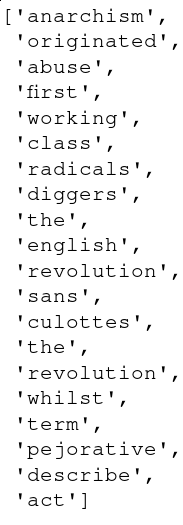
\includegraphics[scale=0.35]{images/text8snippet}
  \end{columns}
\end{frame}

\begin{frame}
\frametitle{Network Architecture} 
\begin{columns}
    \column{0.6\textwidth}
\begin{itemize}
\item Dimension of input and output vectors = 100
\item Context window  = 5
\end{itemize}
    \column{0.6\textwidth}
    \begin{itemize}
    \item Negative Samples = 10 
\item Coded in Pytorch 1.0
\end{itemize}
  \end{columns}
  \bigskip
\begin{columns}
    \column{0.4\textwidth}
    		First 10 pairs of training:
        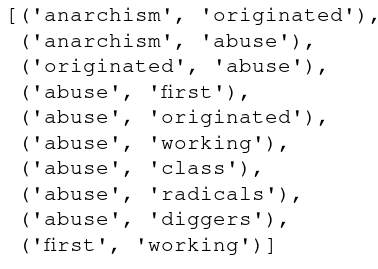
\includegraphics[scale=0.35]{images/pairs_example}    \column{0.6\textwidth}
        Negative Samples:\\
        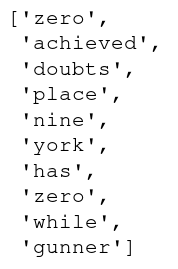
\includegraphics[scale=0.35]{images/neg_samples_example}
  \end{columns}
\end{frame}

\begin{frame}
\frametitle{Optimization process}
Optimization techniques:
\begin{itemize}
\item Advanced Optimizers
\begin{itemize}
\item Momentum
\item Nesterov accellerated Momentum 
\item Adagrad 
\item Adadelta
\item Adam
\end{itemize}
\item Input Shuffling
\end{itemize}
\end{frame}
